%!TEX root = ./icml_2019_sketchmcmc.tex

\begin{figure*}
\centering
\subfigure[]{
	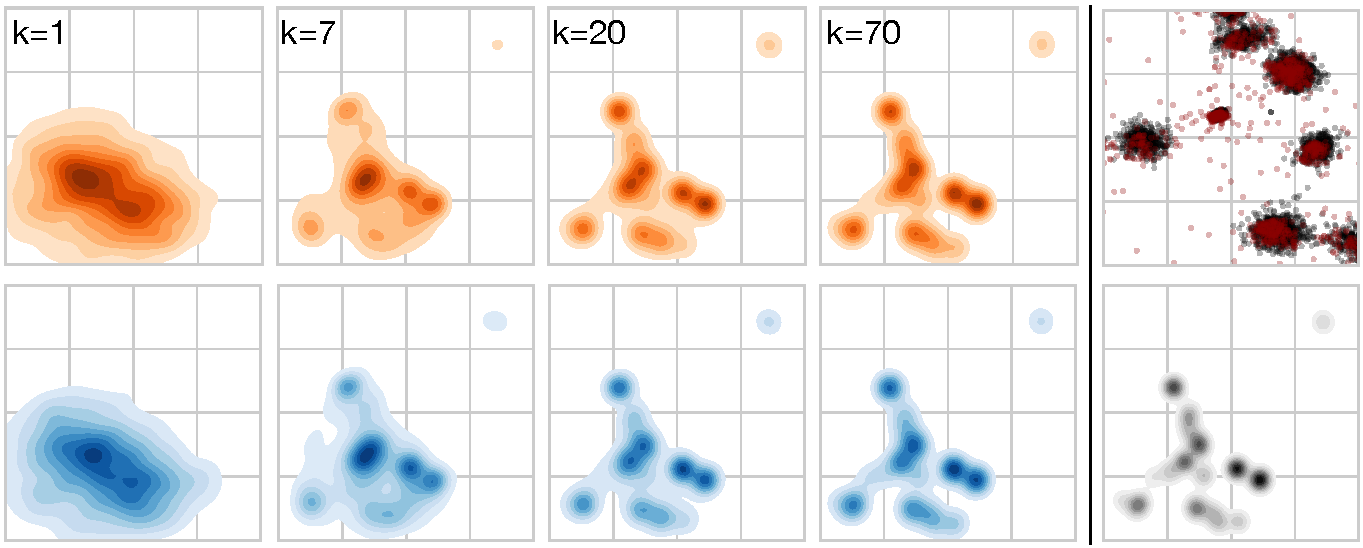
\includegraphics[width=1.25\columnwidth]{gmm_iter.pdf}
	\label{fig:toy_example}
} \hspace{30pt}
\subfigure[]{
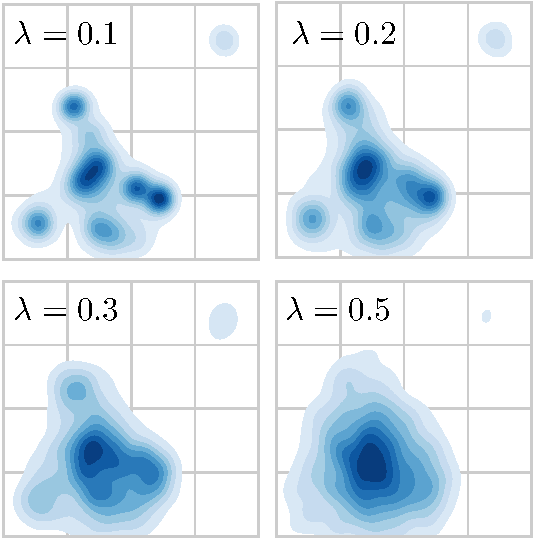
\includegraphics[width=0.49\columnwidth]{gmm_reg.pdf}
\label{fig:lambda_supp}
 }
 % \vspace{-\baselineskip}
\caption{a) \textbf{Left:} Distribution of particles (contour plots) during the estimation (top) and prediction (bottom) stages. \textbf{Right:} (top) Close-up of some generated particles in red superimposed with data points in black. (bottom) Target distribution. b) Influence of the regularization parameter~$\lambda$. }
\label{fig:gmm1}
\end{figure*}

\section{Experiments}


%
In this section, we evaluate the SWF algorithm on a synthetic and a real data setting. Our primary goal is to validate our theory and illustrate the behavior of our non-standard approach, rather than to obtain the state-of-the-art results in IGM. In all our experiments, the initial distribution $\mu_0$ is selected as the standard Gaussian distribution on $\R^d$, we take $Q=100$ quantiles and $N=3000$ particles, which proved sufficient to approximate the quantile functions accurately.


\subsection{Gaussian Mixture Model }
We perform the first set of experiments on synthetic data where we consider a standard Gaussian mixture model (GMM) with $20$ and random parameters. Centroids are taken as sufficiently distant from each other to make the problem more challenging. We generate $P=50000$ data samples in each experiment.

In our first experiment, we set $d=2$ for visualization purposes and illustrate the general behavior of the algorithm. Figure~\ref{fig:toy_example} shows the evolution of the particles through the iterations. Here, we set $N_\theta=30$, $h=1$ and $\lambda=10^{-4}$.
%
We observe that the empirical distribution of the particles converges rapidly to the target distribution. Furthermore, we can see that the QFs, $F^{-1}_{\theta^*_\#\bar{\mu}_{kh}^{N}}$ that are computed with the initial set of particles (so-called the \textit{estimation} stage in Figure~\ref{fig:gmm1}) can be perfectly re-used for new unseen particles in a subsequent \textit{prediction} stage.

% In both cases, we observe two remarkable outcomes: (i) Even when some modes are isolated from the others, SWF is able to capture them successfully and we never observe a mode collapse. This is due to the OT nature of the procedure. (ii) The generated particles do not collapse on the data points, thanks to the entropy regularization.


In our second experiment, we investigate the effect of the level of the regularization $\lambda$. Figure~\ref{fig:lambda_supp}, the distribution of the particles becomes more spread with increasing $\lambda$. This is due to the increment of the entropy, as expected.

\subsection{Experiments on real data}

In a second set of experiments, we test the SWF algorithm on two real datasets. (i) The traditional MNIST dataset that contains 70K binary images corresponding to different digits. (ii) The recently proposed FashionMNIST dataset \cite{xiao2017fashion}, that contains $50000$ gray-scale images. This dataset is advocated as more challenging than MNIST. In all cases, images were interpolated as $32\times 32$, yielding a dimension of $1024$.

In experiments reported in \supp, we found out that directly applying SWF to such high-dimensional data yielded noisy results. To reduce the dimensionality, we trained a standard convolutional autoencoder (AE) on the training set of both dataset (see Figure~\ref{fig:using_ae} and \supp), and the target distribution $\nu$ considered becomes the distribution of the resulting bottleneck features,
with dimension $d$. Particles can be visualized with the pre-trained decoder.
Our goal is to show that SWF permits to directly sample from the distribution of bottleneck features directly, as an alternative to enforcing that distribution to match some prior, as in VAE. In the following, we set $\lambda=0$, $d=48$ and $N_\theta=16000$.

\begin{figure}
\centering
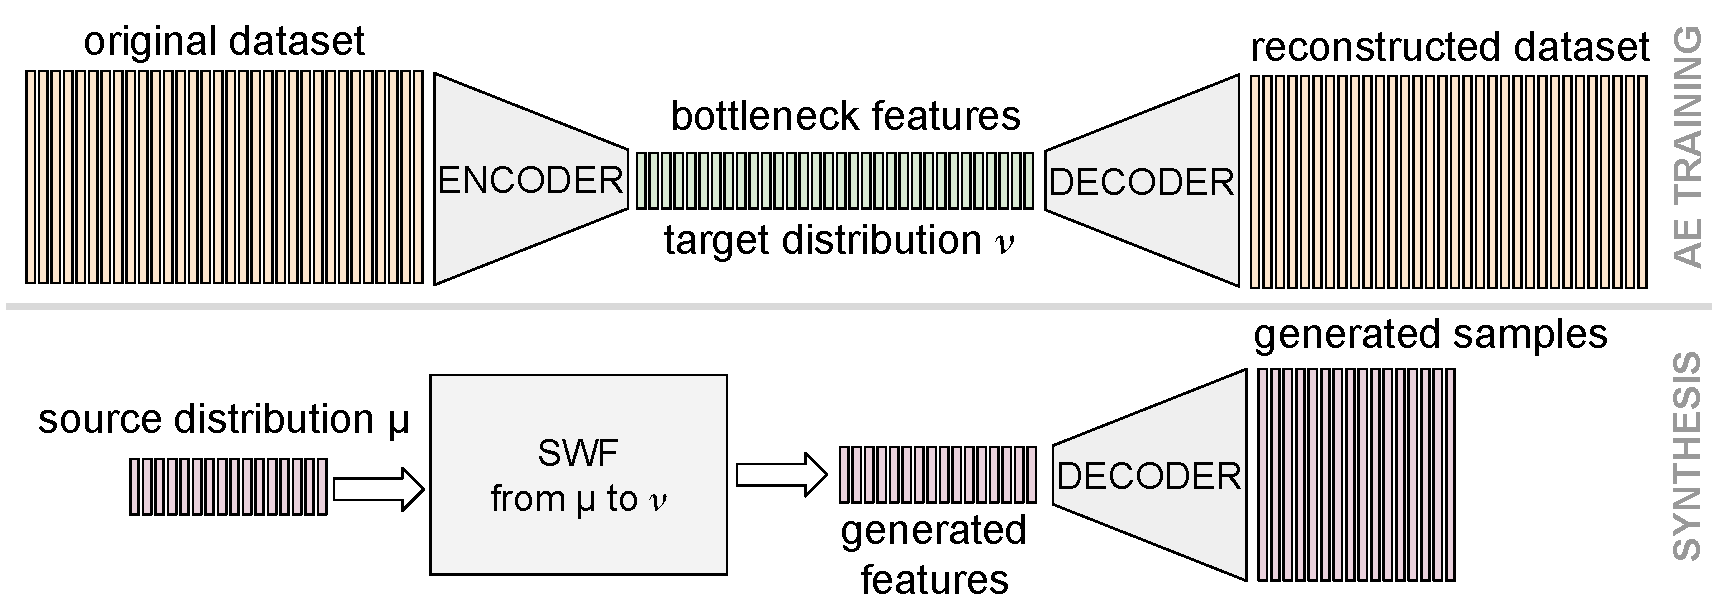
\includegraphics[width=0.99\columnwidth]{figures/generating_bottleneck_features.pdf}
\caption{First, we learn a simple autoencoder. Then, we use SWF to transport random vectors to the distribution of the bottleneck features of the training set. The learned decoder is used for vizualization.}
\label{fig:using_ae}
\vspace{-10pt}
\end{figure}


\begin{figure}
\centering
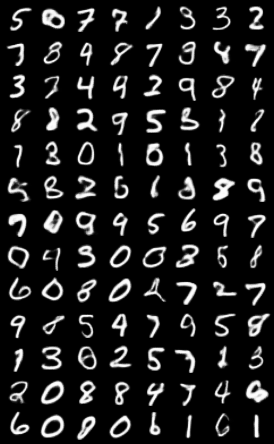
\includegraphics[width=0.45\columnwidth]{figures/MNIST_train_image_1000.png}
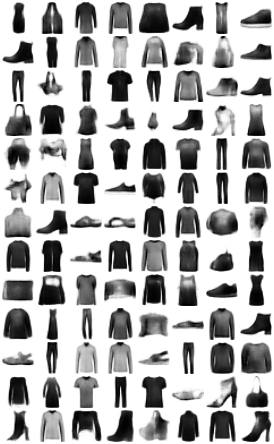
\includegraphics[width=0.45\columnwidth]{figures/FashionMNIST_train_image_1000.png}
\label{fig:samples}
\caption{Samples generated after 200 iterations of SWF to match the distribution of bottleneck features for the training dataset. Visualization is done with the pre-trained decoder.}
% \vspace{-10pt}
\end{figure}


Assessing the validity of IGM algorithms is generally done by visualizing the generated samples. Figures~\ref{fig:samples} shows some particles after a few hundreds iterations of SWF. We can observe they are considerably accurate. Interestingly, the generated samples gradually take the form of either digits or various clothings along the iterations, as illustrated on Figure~\ref{fig:evolution}. In this figure, we also display the closest sample from the original database to check we are not just reproducing training data.

\begin{figure}[]
\centering
\subfigure{
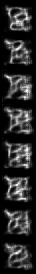
\includegraphics[width=0.06\columnwidth]{figures/MNIST_evolution/train_image_-1.png}
\hspace{0.1cm}

\includegraphics[width=0.06\columnwidth]{figures/MNIST_evolution/train_image_0.png}

\includegraphics[width=0.06\columnwidth]{figures/MNIST_evolution/train_image_2.png}

\includegraphics[width=0.06\columnwidth]{figures/MNIST_evolution/train_image_4.png}
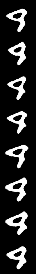
\includegraphics[width=0.06\columnwidth]{figures/MNIST_evolution/train_image_6.png}

\includegraphics[width=0.06\columnwidth]{figures/MNIST_evolution/train_image_8.png}

\includegraphics[width=0.06\columnwidth]{figures/MNIST_evolution/train_image_10.png}

\includegraphics[width=0.06\columnwidth]{figures/MNIST_evolution/train_image_20.png}

\includegraphics[width=0.06\columnwidth]{figures/MNIST_evolution/train_image_50.png}

\includegraphics[width=0.06\columnwidth]{figures/MNIST_evolution/train_image_100.png}

\includegraphics[width=0.06\columnwidth]{figures/MNIST_evolution/train_image_200.png}
\hspace{0.1cm}

\includegraphics[width=0.06\columnwidth]{figures/MNIST_evolution/train_image_match_200.png}
\label{fig:mnist}
}
\hfill
\subfigure{
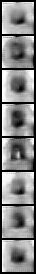
\includegraphics[width=0.06\columnwidth]{figures/FashionMNIST_evolution/train_image_-1.png}
\hspace{0.1cm}

\includegraphics[width=0.06\columnwidth]{figures/FashionMNIST_evolution/train_image_0.png}

\includegraphics[width=0.06\columnwidth]{figures/FashionMNIST_evolution/train_image_2.png}

\includegraphics[width=0.06\columnwidth]{figures/FashionMNIST_evolution/train_image_4.png}
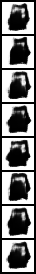
\includegraphics[width=0.06\columnwidth]{figures/FashionMNIST_evolution/train_image_6.png}
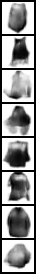
\includegraphics[width=0.06\columnwidth]{figures/FashionMNIST_evolution/train_image_8.png}
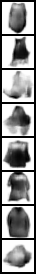
\includegraphics[width=0.06\columnwidth]{figures/FashionMNIST_evolution/train_image_10.png}
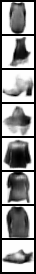
\includegraphics[width=0.06\columnwidth]{figures/FashionMNIST_evolution/train_image_20.png}
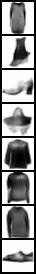
\includegraphics[width=0.06\columnwidth]{figures/FashionMNIST_evolution/train_image_50.png}

\includegraphics[width=0.06\columnwidth]{figures/FashionMNIST_evolution/train_image_100.png}

\includegraphics[width=0.06\columnwidth]{figures/FashionMNIST_evolution/train_image_100.png}
\hspace{0.1cm}
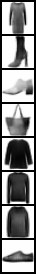
\includegraphics[width=0.06\columnwidth]{figures/FashionMNIST_evolution/train_image_match_200.png}
\label{fig:fashionmnist}
}
% \vspace{-10pt}
\caption{Initial random particles (left), particles through iterations (middle, from 1 to 200 iterations) and closest sample from the training dataset (right), for both MNIST and FashionMNIST.\label{fig:evolution}}
% \vspace{-10pt}
\end{figure}

\begin{figure}[]
\centering
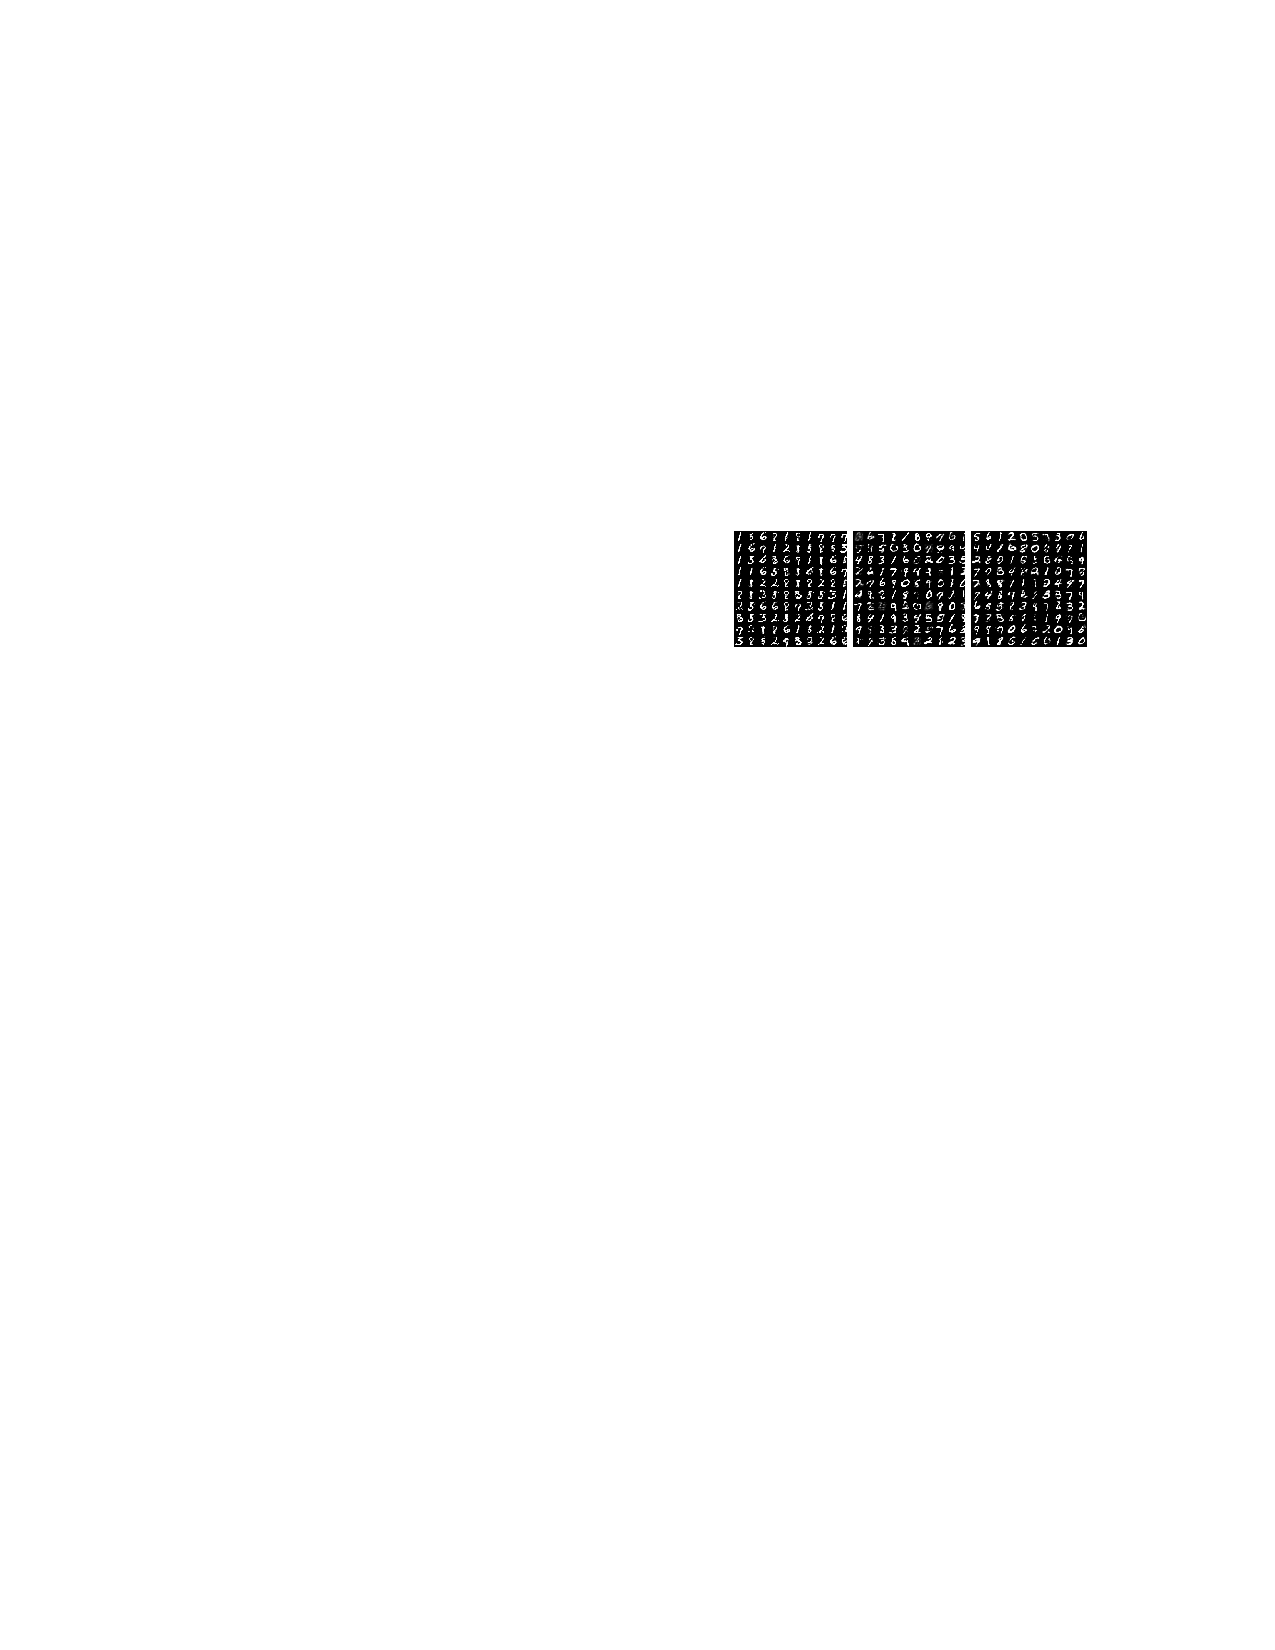
\includegraphics[width=0.99\columnwidth]{mnist_all.pdf}
\caption{Performance of GAN (left), W-GAN (middle), SWG (right) on MNIST. (The figure is directly taken from \cite{deshpande2018generative}.) }
\label{fig:mnistall}
\vspace{-10pt}
\end{figure}

For a visual comparison, we provide the results presented in \cite{deshpande2018generative} in Figure~\ref{fig:mnistall}. These results are obtained by running different IGM approaches on the MNIST dataset, namely GAN \cite{goodfellow2014generative}, Wasserstein GAN (W-GAN) \cite{arjovsky2017wasserstein} and the Sliced-Wasserstein Generator (SWG) \cite{deshpande2018generative}.
%
% in \supp{}, we provide some of the recent results obtained by \cite{deshpande2018generative} on the MNIST dataset.
The visual comparison suggests that the samples generated by SWF is less crisp than the neural network-based approaches, such as \cite{goodfellow2014generative,arjovsky2017wasserstein,deshpande2018generative}.

\begin{figure}
\centering
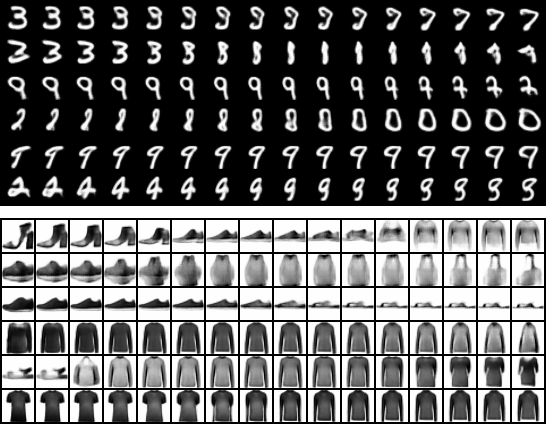
\includegraphics[width=0.95\columnwidth]{figures/interpolations.png}
\label{fig:interpolation}
\caption{Applying a pre-trained SWF on new samples located in-between the ones used for training. Visualization is done with the pre-trained decoder.}
% \vspace{-10pt}
\end{figure}

We also provide the outcome of the pre-trained SWF with samples that are regularly spaced inbetween those used for training. The result is shown in figure \ref{fig:interpolation}. This plot suggests that SWF is a way to interpolate non-parametrically inbetween latent spaces of regular AE.




%On the other hand, another important advantage of SWF is its low computational requirements. The whole experiment on the FashionMNIST requires around $1$ hour of computational time on the CPU of a standard laptop computer, to be compared with the significant resource requirements of the current IGM methods, such GANs and VAEs (typically several days on the same CPU architecture).




















%%% Local Variables:
%%% mode: latex
%%% TeX-master: "aistats_2019_sketchmcmc"
%%% End:
